\chapter{Shapley Values}

\section{Auxiliary Graph}
From the clustered graph a weighted auxiliary graph is defined for each frame, denoted as $G^{aux}$ := ($V$, $E^{aux}$, $w^{aux}$). \\
The vertices of this auxiliary graph are the same as in the original graph $G$, but the edge set is comprised of a subset of edges that only connect vertices belonging to different clusters.
The weight of every edge is calculated by applying Euclidean norm (Formula \ref{formula:normalization}) between pairs of vectors
At least one of these edges in the auxiliary graph will be the edge associated with the origin of motion. \\
Later on, we will see how to choose the correct edge.
\\

Considering, for example, a graph $G$ with 3 clusters (see Figure \ref{fig:graph_g}), we can visualize which edges will be involved in the auxiliary graph (Figure \ref{fig:aux_graph}).
\begin{figure}
  \begin{subfigure}{0.45\textwidth}
    \centering
    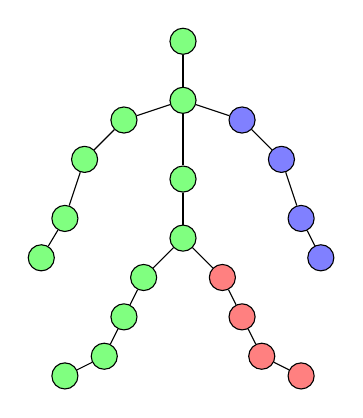
\begin{tikzpicture}
      \node[circle, draw, minimum size=0.1cm] (1) at (3.5,-1.25) [fill=green!50] {};
      \node[circle, draw, minimum size=0.1cm] (2) at (6.5, -1.25) [fill=red!50] {};
      \node[circle, draw, minimum size=0.1cm] (3) at (4,-1) [fill=green!50] {};
      \node[circle, draw, minimum size=0.1cm] (4) at (6, -1) [fill=red!50] {};
      \node[circle, draw, minimum size=0.1cm] (5) at (4.25,-0.5) [fill=green!50] {};
      \node[circle, draw, minimum size=0.1cm] (6) at (5.75,-0.5) [fill=red!50] {};
      \node[circle, draw, minimum size=0.1cm] (7) at (4.5,0) [fill=green!50] {};
      \node[circle, draw, minimum size=0.1cm] (8) at (5, 0.5) [fill=green!50] {};
      \node[circle, draw, minimum size=0.1cm] (9) at (5.5,0) [fill=red!50] {};
      \node[circle, draw, minimum size=0.1cm] (10) at (5,1.25) [fill=green!50] {};
      \node[circle, draw, minimum size=0.1cm] (11) at (3.2, 0.25) [fill=green!50] {};
      \node[circle, draw, minimum size=0.1cm] (12) at (6.75,0.25) [fill=blue!50] {};
      \node[circle, draw, minimum size=0.1cm] (13) at (3.5, 0.75) [fill=green!50] {};
      \node[circle, draw, minimum size=0.1cm] (14) at (6.5, 0.75) [fill=blue!50] {};
      \node[circle, draw, minimum size=0.1cm] (15) at (3.75,1.5) [fill=green!50] {};
      \node[circle, draw, minimum size=0.1cm] (16) at (6.25,1.5) [fill=blue!50] {};
      \node[circle, draw, minimum size=0.1cm] (17) at (4.25,2) [fill=green!50] {};
      \node[circle, draw, minimum size=0.1cm] (18) at (5,2.25) [fill=green!50] {};
      \node[circle, draw, minimum size=0.1cm] (19) at (5.75,2) [fill=blue!50] {};
      \node[circle, draw, minimum size=0.1cm] (20) at (5,3) [fill=green!50] {};  
      \foreach \source/\dest/\label/\xshiftval in {20/18//0, 18/17//0, 18/19//0, 17/15//0, 15/13//0, 13/11//0, 19/16//0, 16/14//0, 14/12//0, 18/10//0, 10/8//0, 8/7//0, 7/5//0, 5/3//0, 3/1//0, 8/9//0, 9/6//0, 6/4//0, 4/2//0}
        \path (\source) edge node[xshift=\xshiftval] {\label} (\dest);
    \end{tikzpicture}
    \caption{Graph $G$}
    \label{fig:graph_g}
  \end{subfigure}
  \hspace{0.01\linewidth}
  \begin{subfigure}{0.45\linewidth}
    \centering
    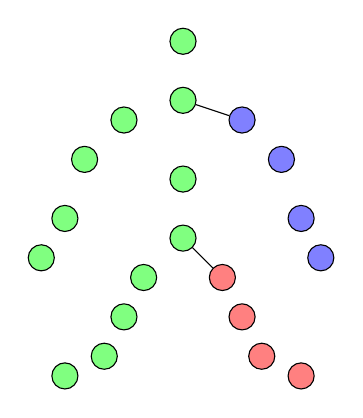
\begin{tikzpicture}
      \node[circle, draw, minimum size=0.1cm] (1) at (3.5,-1.25) [fill=green!50] {};
      \node[circle, draw, minimum size=0.1cm] (2) at (6.5, -1.25) [fill=red!50] {};
      \node[circle, draw, minimum size=0.1cm] (3) at (4,-1) [fill=green!50] {};
      \node[circle, draw, minimum size=0.1cm] (4) at (6, -1) [fill=red!50] {};
      \node[circle, draw, minimum size=0.1cm] (5) at (4.25,-0.5) [fill=green!50] {};
      \node[circle, draw, minimum size=0.1cm] (6) at (5.75,-0.5) [fill=red!50] {};
      \node[circle, draw, minimum size=0.1cm] (7) at (4.5,0) [fill=green!50] {};
      \node[circle, draw, minimum size=0.1cm] (8) at (5, 0.5) [fill=green!50] {};
      \node[circle, draw, minimum size=0.1cm] (9) at (5.5,0) [fill=red!50] {};
      \node[circle, draw, minimum size=0.1cm] (10) at (5,1.25) [fill=green!50] {};
      \node[circle, draw, minimum size=0.1cm] (11) at (3.2, 0.25) [fill=green!50] {};
      \node[circle, draw, minimum size=0.1cm] (12) at (6.75,0.25) [fill=blue!50] {};
      \node[circle, draw, minimum size=0.1cm] (13) at (3.5, 0.75) [fill=green!50] {};
      \node[circle, draw, minimum size=0.1cm] (14) at (6.5, 0.75) [fill=blue!50] {};
      \node[circle, draw, minimum size=0.1cm] (15) at (3.75,1.5) [fill=green!50] {};
      \node[circle, draw, minimum size=0.1cm] (16) at (6.25,1.5) [fill=blue!50] {};
      \node[circle, draw, minimum size=0.1cm] (17) at (4.25,2) [fill=green!50] {};
      \node[circle, draw, minimum size=0.1cm] (18) at (5,2.25) [fill=green!50] {};
      \node[circle, draw, minimum size=0.1cm] (19) at (5.75,2) [fill=blue!50] {};
      \node[circle, draw, minimum size=0.1cm] (20) at (5,3) [fill=green!50] {};  
      \foreach \source/\dest/\label/\xshiftval in {18/19//0, 8/9//0}
        \path (\source) edge node[xshift=\xshiftval] {\label} (\dest);
    \end{tikzpicture}
    \caption{Auxiliary graph $G^{aux}$}
    \label{fig:aux_graph}
  \end{subfigure}
\end{figure}


A cooperative TU game on the weighted auxiliary graph is constructed. \\
The value \textit{c}($V'$) associated with a generic coalition $V'$ is chosen as the summation of all the weights in the weighted auxiliary graph $G^{aux}$ associated with
the physical edges belonging to the subgraph of the auxiliary graph that is induced by $V'$.\\
More precisely, the characteristic function is chosen as follows:


\begin{center}
    \begin{equation}
    c(V') = \sum_{v, \hat{v} \in V', \hat{v} \in N^{aux}(v)} w^{aux}(e^{aux}_{v, \hat{v}})
    \end{equation}
\end{center}
    
\begin{center}
    \begin{equation}
    \phi(i) := \sum_{V'\subseteq V\setminus \{i\}} \frac{|V'|! (|V|-|V'|-1)!}{|V|!} (c(V' \cup \{i\}) - c(V'))
    \end{equation}
\end{center}
    